% DRAFT 2 — MINIMALIST (poster2.tex). Build: pdflatex poster2.tex (twice)
\documentclass[final]{beamer}
\usepackage[orientation=landscape, size=a0, scale=0.84]{beamerposter}
\usepackage[T1]{fontenc}
\usepackage[utf8]{inputenc}
\usepackage[scaled=0.92]{helvet}
\renewcommand{\familydefault}{\sfdefault}
\usepackage{lmodern}
\usepackage{amsmath,amssymb}
\usepackage{booktabs}
\usepackage{graphicx}
\usepackage{ragged2e}
\usepackage{xcolor}
\usepackage{tikz}
\usetikzlibrary{shapes,shadows,arrows.meta,positioning,calc}
\usepackage{pgfplots}
\pgfplotsset{compat=1.18}
\setlength{\overfullrule}{4pt}
\definecolor{navy}{HTML}{0E2A47}
\definecolor{navy2}{HTML}{14456E}
\definecolor{accent}{HTML}{0091B3}
\definecolor{accent2}{HTML}{E27A1E}
\definecolor{panel}{HTML}{F2F6FA}
\definecolor{panel2}{HTML}{E4EDF6}
\definecolor{good}{HTML}{1E7B4F}
\definecolor{bad}{HTML}{B13325}
\definecolor{gold}{HTML}{C79A2B}
\setbeamercolor{block title}{fg=white, bg=navy}
\setbeamercolor{block body}{fg=black!88, bg=panel}
\setbeamerfont{block title}{size=\Large, series=\bfseries}
\setbeamerfont{block body}{size=\Large}
\setbeamercolor{itemize item}{fg=accent}
\setbeamertemplate{itemize item}{\raisebox{0.35ex}{\small$\blacktriangleright$}}
\setlength{\leftmargini}{1.1cm}
\setbeamertemplate{itemize/enumerate body begin}{\setlength{\itemsep}{0.06cm}}
\newlength{\blocklskip}\setlength{\blocklskip}{0.55cm}
\newlength{\blockrskip}\setlength{\blockrskip}{0.55cm}
\setbeamertemplate{block begin}{%
  \par\vskip0.28cm%
  \begin{beamercolorbox}[wd=\linewidth,leftskip=0.5cm,rightskip=0.5cm,sep=0.25cm]{block title}%
    \usebeamerfont*{block title}\insertblocktitle%
  \end{beamercolorbox}%
  {\nointerlineskip\vskip-0.5pt}%
  \usebeamerfont{block body}%
  \begin{beamercolorbox}[wd=\linewidth,leftskip=\blocklskip,rightskip=\blockrskip,vmode]{block body}%
    \setlength{\linewidth}{\dimexpr\linewidth-\blocklskip-\blockrskip\relax}%
    \setlength{\hsize}{\linewidth}\setlength{\textwidth}{\linewidth}\setlength{\columnwidth}{\linewidth}%
    \setlength{\parskip}{0.10cm}\justifying%
}
\setbeamertemplate{block end}{\end{beamercolorbox}\vspace*{0.05cm}}
\setbeamertemplate{navigation symbols}{}
\setbeamertemplate{headline}{}
\setbeamertemplate{footline}{}
\setbeamersize{text margin left=1.0cm, text margin right=1.0cm}
\newcommand{\hl}[1]{\textbf{\textcolor{navy2}{#1}}}
\newcommand{\code}[1]{{\ttfamily\small #1}}
\newcommand{\figcap}[1]{{\centering\small\itshape\color{black!62} #1\par}}
\newcommand{\kpi}[3]{%
  \begin{minipage}[t]{0.235\linewidth}\centering
    {\color{#3}\fontsize{30}{30}\selectfont\bfseries #1}\\[0.08cm]
    {\small\bfseries #2}%
  \end{minipage}%
}
\tikzset{
  laybox/.style={rounded corners=14pt, draw=navy, line width=2.5pt, fill=white,
    minimum width=13.2cm, minimum height=15.5cm, align=center, text width=12.4cm,
    drop shadow={shadow xshift=3pt, shadow yshift=-3pt, opacity=0.18}},
  laytitle/.style={fill=navy, text=white, font=\bfseries\Large, rounded corners=8pt,
    minimum width=11.2cm, minimum height=1.6cm, align=center, text width=10.8cm},
  arrowbig/.style={{Stealth[length=14pt,width=10pt]}-, line width=4pt, draw=accent},
  arrowthin/.style={{Stealth[length=11pt,width=8pt]}-, line width=3pt, draw=good},
}
\begin{document}
\begin{frame}[t]
\begin{beamercolorbox}[wd=\textwidth,leftskip=1.2cm,rightskip=1.2cm,sep=0.55cm]{block title}
\centering
{\fontsize{44}{46}\selectfont\bfseries Fusing LLM Semantic Repair with Genetic Programming for Robust Alpha Discovery\par}
\vspace{0.25cm}
{\Large G.S.K. Raghav Anand \textbullet\ Hitesh Rasineni \textbullet\ G Siva Sanjay Reddy \textbullet\ K Dharma Teja \textbullet\ VIT-AP University \textbullet\ IEEE Access manuscript\par}
\vspace{0.2cm}
{\large\itshape Vanilla quant models break out-of-sample. A regime-aware GP + local-LLM repair loop fixes that --- S\&P 500 Sharpe decay cut from \textbf{$-35\%$ to $-7\%$}, China's from $-92\%$ to $-47\%$, and no candidate tree is ever thrown away --- the whole loop costs one monthly pass on a single workstation.}
\end{beamercolorbox}
\vskip0.3cm
\begin{beamercolorbox}[wd=\textwidth,leftskip=0.8cm,rightskip=0.8cm,sep=0.35cm]{block body}
\centering
\kpi{10.6\%}{net return (peak)}{good}\hfill
\kpi{0.65}{net Sharpe}{navy2}\hfill
\kpi{$-7\%$}{S\&P decay (was $-35\%$)}{good}\hfill
\kpi{+18\%}{over quant ceiling}{accent2}\\[0.1cm]
{\small NSE Nifty 50 2002--2025 (23 yrs) \textbullet\ validated on S\&P 500 + SSE \textbullet\ costs 20+10 bps, cap INR 50 Cr \textbullet\ local Llama-3.2-3B + Gemma-2-2B, \$0 inference \textbullet\ one monthly rebalance, judged and repaired in minutes}
\end{beamercolorbox}
\vskip0.2cm
\begin{columns}[t,onlytextwidth]
\column{0.245\linewidth}
\begin{block}{0 Objectives}
\begin{itemize}
  \item \hl{Primary:} discover symbolic ranking formulas that maximise forward risk-adjusted return across regimes while cutting out-of-sample decay.
  \item \hl{Secondary:} keep every candidate via repair-not-reject; stay cheap (local 3B/2B, \$0) and tradable (costs + cap priced in).
  \item \hl{Validate:} NSE Nifty 50 2002--2025, transfer to S\&P 500 + SSE with one fixed setup.
\end{itemize}
\end{block}
\begin{block}{1 Problem in 30 seconds}
\begin{itemize}
  \item Quant factors \hl{decay}: top-1000 anomalies lose about 32\% after publication; GP memorises noise.
  \item Old LLM+GP hybrids \hl{delete} bad formulas and lose diversity.
  \item Fix: \hl{repair, don't reject} --- rewrite only the truly nonsensical (score 2 or less).
  \item Deletion is expensive: a dropped tree takes its partial signal with it; a thinner pool overfits one lucky regime.
  \item Local 3B/2B models make the judge cheap: \$0 API cost, prompts stay on-workstation, latency fits monthly rebalance.
  \item Claim stays narrow: repair lifts out-of-sample stability, not in-sample fit; risk budget never widens.
\end{itemize}
\end{block}
\begin{block}{2 What each layer does}
\begin{itemize}
  \item \hl{AFM (slow):} news mood + PE/ROE/EPS/BV gives a bull/bear prior. It drifts over weeks, so one noisy headline never flips it.
  \item \hl{HMM (fast):} 2-state volatility filter: calm to trend, turbulence to reversals + quality (Baum--Welch + Viterbi, daily).
  \item \hl{GP (inventor):} 500 trees, depth max 6, Sharpe-minus-complexity fitness; bloat is charged from generation one.
  \item \hl{LLM (editor):} Llama rates economics 1--5; Gemma rewrites failures from a closed vocabulary ($L\le5$ typed edits max).
  \item \hl{Guards:} repaired trees must pass AST + validation ranges before re-entering; failures never replace parents.
  \item \hl{Settings:} FinBERT $\tau=0.5$; GP pop 500, depth 6; dollar-neutral top/bottom-15\%, monthly rebalance; identical on Nifty, S\&P, SSE.
\end{itemize}
\end{block}

\begin{block}{4 Decay cut in half (Sharpe)}
Out-of-sample Sharpe vs the in-sample peak (3 engines/market): structure that survives the test window bleeds less. Conditioning helps, repair helps more.\par\vspace{0.2cm}
\begin{minipage}{\linewidth}\centering
{\footnotesize
\setlength{\tabcolsep}{0.12cm}\renewcommand{\arraystretch}{1.25}
\begin{tabular}{@{}lcc@{}}
\toprule
\textbf{Market / engine} & \textbf{OOS Sharpe} & \textbf{Decay} \\
\midrule
S\&P Vanilla GP & 0.905 & \textcolor{bad}{\bfseries -35.03\%} \\
S\&P HMM-GP & 0.974 & -20.71\% \\
S\&P \textbf{LLM-GP (ours)} & \textbf{1.075} & \textcolor{good}{\bfseries -6.77\%} \\
\midrule
SSE Vanilla GP & 0.035 & \textcolor{bad}{\bfseries -92.08\%} \\
SSE HMM-GP & 0.232 & -63.28\% \\
SSE \textbf{LLM-GP (ours)} & \textbf{0.067} & \textcolor{good}{\bfseries -46.68\%} \\
\bottomrule
\end{tabular}\par}
\vspace{0.2cm}
{\raggedright\small\itshape\color{black!62} S\&P decay -35.03\% to -6.77\%; China -92.08\% to -46.68\%. Vanilla GP overfits; conditioning removes part, repair removes the rest. SSE level (0.067) stays small, so the claim there is halved decay, not a large Sharpe.\par}
\end{minipage}
\end{block}
\column{0.505\linewidth}
\begin{block}{2b Loop + stability (how it runs, why it holds)}
GP loop: AFM prior + HMM state $\to$ fitness (Sharpe $-$ complexity) $\to$ Llama judge (1--5) $\to$ Gemma repair ($S\le2$, closed vocab, $L\le5$) $\to$ recompile, back into evolution. Trees scoring 3--5 pass untouched, so the editor spends compute only where the economics is broken. Zero attrition: every repair compiles, the pool never drops below its 500 trees, and nothing is discarded for looking unusual --- only for scoring low.
\par\centering
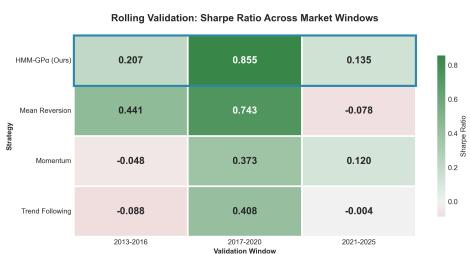
\includegraphics[width=0.52\linewidth,keepaspectratio]{images/28656a9cc9f26a4ffd2ce0ab7611324d8cd0fff6192ee9abf348a58dd50cc0a7.jpg}
\par\figcap{Rolling-window Sharpe stays positive (0.855) in turbulent 2017--20 where momentum + trend turn negative. Regime specialists, not one average model: every rolling window is judged on its own regime, so a calm 2013--16 never has to average out a hostile 2017--20.}
\end{block}
\begin{block}{3 System architecture (paper Fig.~1, middle)}
\centering
{\normalsize\itshape\color{black!70} Left: mine candidates from data + regimes. Right: repair --- never delete --- what the judge rejects. Lower: fuse, size, execute.\par}
\vspace{0.25cm}
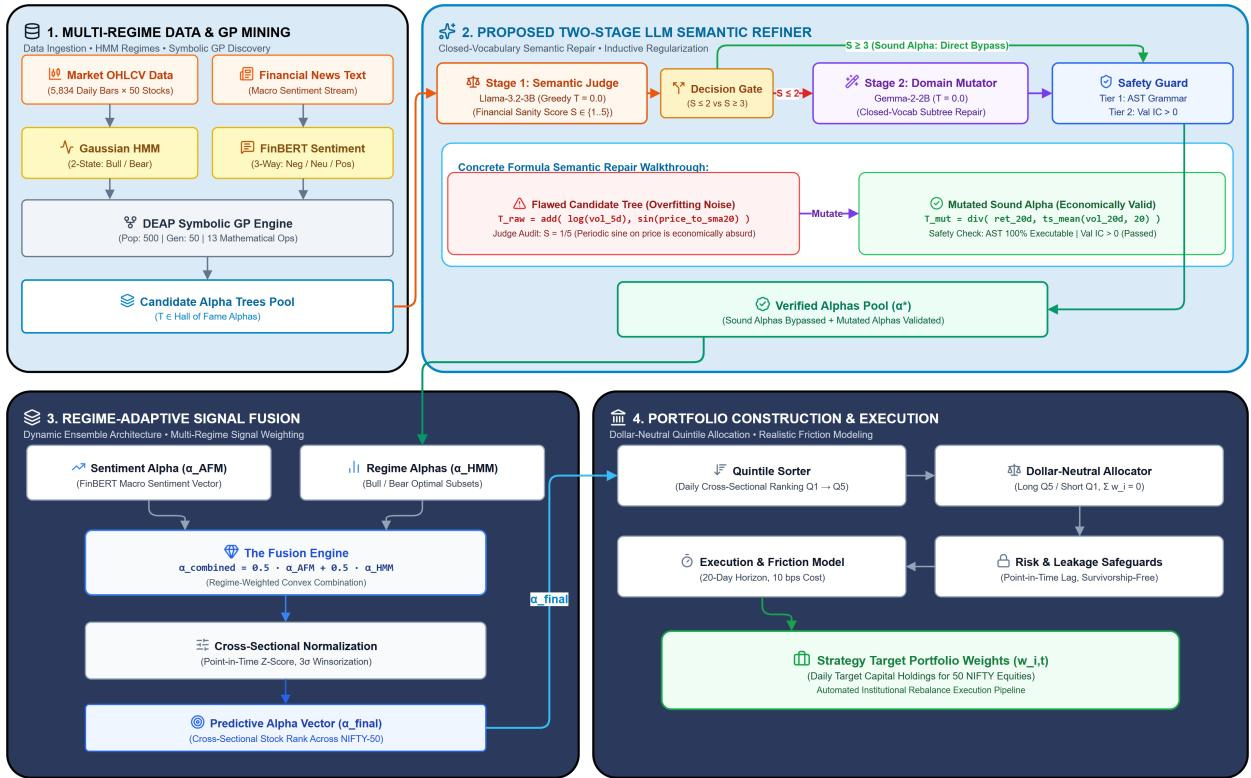
\includegraphics[width=0.98\linewidth,keepaspectratio]{images/38de923ab8b5dcfc8845af49392f1122074f030c0adba45a84530c30bf42c1bf.jpg}
\par\figcap{Figure 1. Dual two-stage framework: (1) regime-aware factor engine (AFM macro + HMM states + regime GP); (2) Two-Stage LLM Refiner (Llama-3B judge, Gemma-2B closed-vocab repair) behind AST + validation guards --- mine, judge, repair, then build the dollar-neutral book.}
\end{block}
\column{0.245\linewidth}
\begin{block}{5 What the machine rediscovers (\mbox{feature} mix)}
\centering
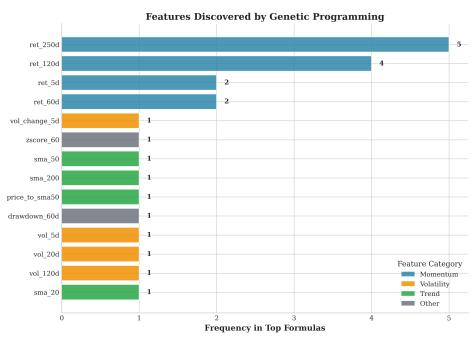
\includegraphics[width=0.62\linewidth,keepaspectratio]{images/97b82991ea2743e616388671ed37ff6bea3cc310277e70b8b60047cb29f427af.jpg}
\par\figcap{Feature mix of top alphas (paper Fig.~6): intermediate momentum + volatility scalers dominate. Each bar counts appearances of that feature in the top-ranked formulas: a trend term you can hold in calm regimes plus a scaler that trims size when vol rises, with reversals + quality for stress. The categories stay classical (trend, momentum, volatility, quality), so every repaired formula still reads like something a desk would write. Because the inputs stay classical, the repair step can never smuggle in data the GP never saw.}
\end{block}
\begin{block}{6 Read this and leave (5-min \mbox{summary})}
\begin{itemize}
  \item \hl{Robust every year:} positive Sharpe 2019--25 incl.\ COVID (-14.8\% DD vs -38.5\% momentum).
  \item \hl{Deployable:} about \$250M capacity; 20+10 bps costs priced in, INR 50 Cr cap.
  \item \hl{Cheap to run:} one monthly pass on a single workstation --- local 3B/2B models, no cloud API, \$0 inference.
  \item \hl{Where it wins:} decay control --- S\&P keeps 93\% of its backtest Sharpe, SSE keeps about half instead of a tenth.
  \item \hl{Honest limits:} the SSE level (0.067) is still small, and transfer is tested on one US plus one Chinese index.
  \item \hl{Next:} NSE 500, LoRA-Gemma, multi-agent judges.
\end{itemize}
\begin{beamercolorbox}[wd=\linewidth,leftskip=0.35cm,rightskip=0.35cm,sep=0.3cm]{block title}
\centering\Large\bfseries Take-away: semantic repair is a free regulariser, India to US to China, at zero inference cost.
\end{beamercolorbox}
\end{block}
\begin{block}{7 Repair example + wealth curve + regimes (one glance)}
Before (1/5): \code{add(log(vol\_5d), sin(p\_to\_sma20))} --- sine on prices is noise: it oscillates with no economic channel, so it fits one window and dies in the next. After (4/5): \code{div(ret\_20d, ts\_mean(vol\_20d,20))} --- return scaled by its own trailing volatility: risk-adjusted momentum, the line a quant desk would write by hand. Rank IC $-0.012 \to +0.038$; 100\% repairs compile, zero crashes over 1,729 days. Both edits stay inside the original operator set, so no new primitive has to be back-tested.\\[0.15cm]
\noindent\begin{minipage}[t]{0.49\linewidth}\centering
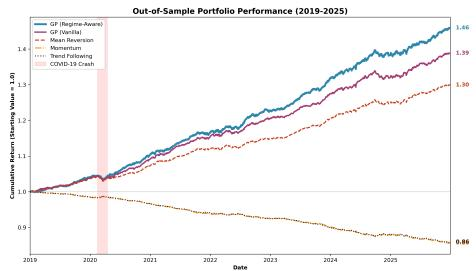
\includegraphics[width=\linewidth,keepaspectratio]{images/ed7d3491c0ec3faa565111046b72b92898718e516bf5ea024476263ee826a05c.jpg}
\\{\small\itshape Wealth 2019--25 compounds through bull + bear while a plain momentum book gives back $-40.65\%$ at its worst.\par}
\end{minipage}\hfill
\begin{minipage}[t]{0.49\linewidth}\centering
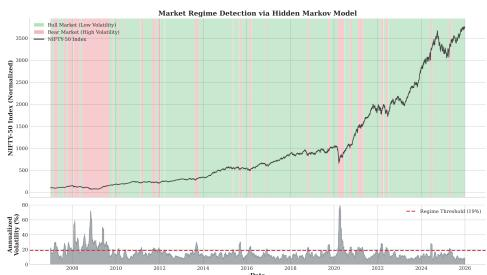
\includegraphics[width=\linewidth,keepaspectratio]{images/33f0cbdd4e18c1897be25763a9a2422f0e044cbf536822f96ca1ea48c66eb838.jpg}
\\{\small\itshape HMM: State 0 calm expansion vs State 1 turbulence (COVID-2020, tightening-2022); stickiness 0.994/0.983 --- the model rarely flips states, so the routing signal stays stable.\par}
\end{minipage}
\figcap{Repair turns nonsense into economics; regime routing is why wealth survives shocks. Read together: cleaner operators on top, regime-aware routing below, one smooth equity curve at the end.}
\end{block}
\end{columns}
\vskip0.25cm
\begin{beamercolorbox}[wd=\textwidth,sep=0.3cm]{block body}
{\small\raggedright
\textbf{Refs:} Kakushadze 101 Alphas (2016) \textbullet\ AlphaAgent arXiv:2502.16789 \textbullet\ TEDE (2026) \textbullet\ DEAP JMLR \textbullet\ Hamilton (1989) McLean (2016) \textbullet\ Almgren--Chriss (2000).
NSE 50 2002--25; S\&P 500 + SSE transfer test. Draft 1 (poster.pdf) is the full version behind every number shown above.
}
\end{beamercolorbox}
\end{frame}
\end{document}
